
%(BEGIN_QUESTION)
% Copyright 2011, Tony R. Kuphaldt, released under the Creative Commons Attribution License (v 1.0)
% This means you may do almost anything with this work of mine, so long as you give me proper credit

Det er vanlig praksis å koble en antenne til en radiosender/mottaker (transceiver) via en transmisjonslinje når antennen må plasseres høyt for å få god mottakskvalitet. I dette eksemplet brukes en radiotransceiver til å overføre måledata for naturgassmengde fra en flowcomputer til en fjern lokasjon, som del av et SCADA-system for naturgassrørledningen. Antennen er plassert på toppen av en trestolpe for bedre signalstyrke enn om den stod ved bakkenivå:

$$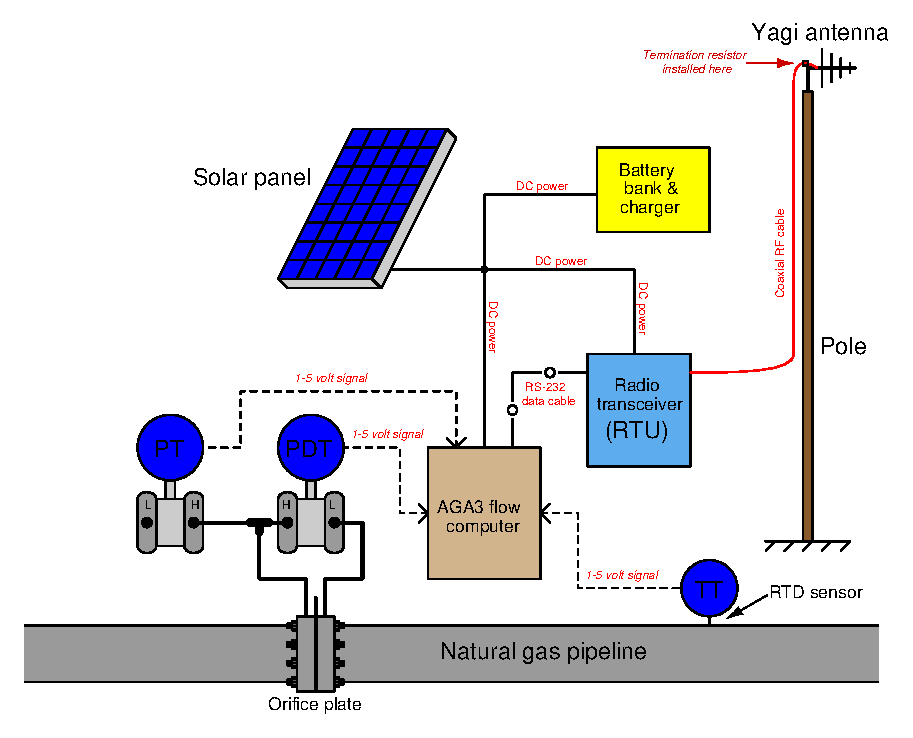
\includegraphics[width=15.5cm]{i01357x01.eps}$$

I denne installasjonen er transmisjonslinjen en 20 fot lang 50 $\Omega$ koaksialkabel. Siden reflekterte signaler er uønsket i ethvert transmisjonslinjesystem, monterte teknikeren som installerte systemet også en 50 $\Omega$ {\it termineringsmotstand} i antenneenden av kabelen, parallelt med antennen.

Var installasjon av denne termineringen en god idé, eller ikke? Begrunn svaret.

\vskip 20pt \vbox{\hrule \hbox{\strut \vrule{} {\bf Forslag til sokratisk diskusjon} \vrule} \hrule}

\begin{itemize}
\item{} Forklar hvordan en TDR kan brukes til å kontrollere transmisjonslinjen for korrekt terminering.
\item{} For de som har studert gassmengdemåling: Hva betyr {\it AGA3}, og hvorfor er det {\it tre} prosesstransmittere koblet til flowcomputeren?
\item{} Forklar hva et ``SCADA''-system er, og hvilken funksjon det fyller.
\item{} Det er ganske vanlig å finne analoge transmittere i solcelledrevne SCADA-overvåkingssteder som bruker {\it spennings}-signaler i stedet for {\it strøm}-signaler, som er vanligere i industrielle (prosessanlegg-)applikasjoner. Grunnen til dette er å redusere effektforbruket. Forklar hvordan bruk av spenningssignaler reduserer effektforbruket sammenlignet med strømsignaler.
\item{} Er dette et reelt eksempel på en ``SCADA''-node, eller passer det bedre å karakterisere det som en {\it telemetri}-node? Begrunn svaret.
\end{itemize}

\underbar{file i01357}
%(END_QUESTION)





%(BEGIN_ANSWER)

Det er overhodet ikke behov for en termineringsmotstand i enden av en transmisjonslinje som avsluttes i en antenne.

%(END_ANSWER)





%(BEGIN_NOTES)

Ikke sett terminator på kabelen, fordi den vil absorbere signalpulser! I stedet vil du at selve antennen skal være det dissiperende elementet. Hvis antennen er riktig tilpasset kabelen, vil den terminere kabelen godt nok til å minimere signalrefleksjoner i kabelen, fordi antennen oppfører seg som en dissipativ last.

%INDEX% Electronics review: antennas
%INDEX% Electronics review: characteristic impedance of transmission line
%INDEX% Electronics review: surge impedance of transmission line

%(END_NOTES)

